\documentclass{article}
\usepackage{spconf,amsmath,graphicx}

\usepackage[breaklinks=true,colorlinks,bookmarks=false]{hyperref}

\newcommand{\todo}[1]{\textcolor{red}{todo: {\em #1}}}
\newcommand{\figref}[1]{Figure~\ref{fig:#1}}

% Title.
% ------
\title{Deep Methods for Estimating Transient Scene Properties}
%
% Single address.
% ---------------
\name{}
\address{University of Kentucky}
%
% For example:
% ------------
%\address{School\\
%	Department\\
%	Address}
%
% Two addresses (uncomment and modify for two-address case).
% ----------------------------------------------------------
%\twoauthors
%  {A. Author-one, B. Author-two\sthanks{Thanks to XYZ agency for funding.}}
%	{School A-B\\
%	Department A-B\\
%	Address A-B}
%  {C. Author-three, D. Author-four\sthanks{The fourth author performed the work
%	while at ...}}
%	{School C-D\\
%	Department C-D\\
%	Address C-D}
%
\begin{document}
%\ninept
%
\maketitle
%
\begin{abstract}
	
	\todo{Write me}
  Deep learning has been used to obtain state of the art results in
  problems ranging from object classification, object detection, and
  scene classification. We evaluate the use of deep learning to
  predict more subtle visual scene aspects, such as the weather, the
  season, and subjective scene properties. 

\end{abstract}
%
\begin{keywords}
	deep learning, transient attributes
\end{keywords}

\section{Introduction}
\todo{Write me}
% general intro to the problem and why it is important

% what do we propose to do? 
We propose a method for predicting transient attributes on images using
deep convolutional neural networks.  These networks achieve better 
predictions for most of the attributes and predict the attributes
faster than the methods proposed by Laffont\cite{Laffont14} et al.
% how do we evaluate this?

We evaluate the proposed method on several benchmarks.  The first 
benchmark is the Transient Attributes Dataset\cite{Laffont14}.  This 
is the standard benchmark for transient attributes in images. 

% what we can do now that we have this?

% key contributions: repeat what was said above in bullet point form
The key contributions of this work are:
\begin{itemize}

  \item comparison of several deep learning network architectures for
    the problem

  \item state-of-the-art results on two benchmark datasets (transient
    attributes and two class weather)

  \item something with running it on webcam data?

\end{itemize}

\subsection{Related Work}

\todo{Write me}

Previous approaches to this problem include (some general description
of previous approaches and how they compare to what we propose).

List of related papers:
\begin{itemize}

  \item add citation and one sentence description of what it does, one
    sentence description of how it is different from what we do, maybe
    something about how they evaluate.

\end{itemize}

\section{Estimating Transient Attributes Using CNNs}

\subsection{Transient Attributes Dataset}
\indent

We used the dataset created by Laffont\cite{Laffont14} et al. to train our 
networks. The dataset contains images from outdoor webcams in the  
Archive of Many Outdoor Scenes\cite{jacobs07amos} and the Webcam Clip Art 
Dataset\cite{lalondesig09}.  The webcams span a wide range of outdoor scenes,
from urban regions to wooded, mountainous regions. Each webcam has 60-120 
representative images that feature variations in weather, lighting conditions, 
etc.  The images are high resolution and are aligned to a reference frame 
through a homography warp with manually specified correspondences.  The final
dataset consists of 8571 images from 101 webcams.

\subsection{Recap of CNNs}

\todo{add a summary of the different models, and how they were
trained, include a bibtex citation for each one.}

\textbf{Caffenet:} Caffenet is the reference network provided with 
Caffe\cite{caffe14}.  It was trained on 1.2 million images from the 
ILSVRC-2012\cite{ILSVRCarxiv14} challenge and is based on the architecture from 
the NIPS 2012 paper by Krizhevsky\cite{caffenetnips12} et al.  This network has 
8 learned layers, five convolutional layers and three fully-connected layers.  
It was trained on parts of the ImageNet dataset used in the 
ILSVRC-2010\cite{ILSVRCarxiv14} challenge.  This network was originally trained 
for object classification, but works well for other problems. For our application, 
we finetuned the final layer of Caffenet and changed the output of the final 
layer to be 40 (one output for each attribute).

\textbf{Places} The Places205-CNN architecture is the Caffenet network retrained on 
the Places Database\cite{zhou2014places}.  The Places205-CNN was trained on 2.5
million randomly selected images with labels in 205 categories from the Places 
Database.  We fine-tuned the final layer of Places205-CNN using the weights from the
pretrained network model provided by Zhou\cite{zhou2014places} et al.

\textbf{Hybrid:} The Hybrid-CNN architecture is the Caffenet network retrained on
a combination of the Places Database\cite{zhou2014places} and images from the 
training data of ILSVRC-2012\cite{ILSVRCarxiv14} challenge.  The full training set
contained 205 scene categories from the Places Database and 978 object categories
from ILSVRC-2012 totaling about 3.6 million images.  We fine-tuned the last 
layer of Hybrid-CNN using the weights from the pretrained network model provided by 
Zhou\cite{zhou2014places} et al.

\subsection{Description of how we train ours}
\indent

To train our networks, we use the Caffe\cite{caffe14} deep learning 
framework. We finetuned the last layer of each of the networks using the 
holdout split in the transient attributes dataset.  This train/test split uses
the data from 81 webcams for training and the data from 20 separate 
webcams for testing.  Data from webcams in the training set does not
appear in the testing set using the holdout split.  This is contrary to 
the random train/test split.  

\subsection{Deep Network Visualization}

\todo{pictures of what the network looks like\dots highlighting how it
is different from those trained for other purposes... probably
focusing on the one or two that work the best}

\section{Evaluation}

\todo{caffenet works the best, so: caffenet vs. places, caffenet vs. hybrid.
			make those relative error plots to show where caffenet is working better}

\figref{sort} shows the average errors from Caffenet for each attribute
in a sorted graph.  The attributes where Caffenet performed best are towards
the bottom of the graph and the attributes where Caffenet performed
worst are on the top of the graph. \figref{relerr} and \figref{compare} 
compare this performance to the performance of Laffont et al.

\figref{compare} shows the average errors from Caffenet, Places205-CNN, Hybrid-CNN
and Laffont et al. for each attribute in the dataset.  The green bars represent the 
average errors from Laffont et al., the blue bars represent the average errors from 
Caffenet, the red bars represent the average errors from Places205-CNN, and the 
yellow bars represent the error from Hybrid-CNN. Caffenet performs best on more than
half of the attributes and is the best performing CNN that we trained.  Caffenet has 
the lowest average error for most of the attributes.

\figref{relerr} shows the relative error between our method using Caffenet
and the method presented in \cite{Laffont14}.  The average relative error 
for each attribute using the method in \cite{Laffont14} was subtracted from
the average relative error using Caffenet.  A negative value means Caffenet
had a smaller error and a positive value means \cite{Laffont14} had a smaller
error.  For example, the difference between the two methods on the attribute
night was around 3.2 percentage points, with Caffenet having the smaller 
error.

 
 
%Suggested plots:
%\begin{itemize}
%
%  \item summary results you have already shown
%
%  \item example good results, and plausible bad results
%
%\end{itemize}


\begin{figure}[t]
	\centering
		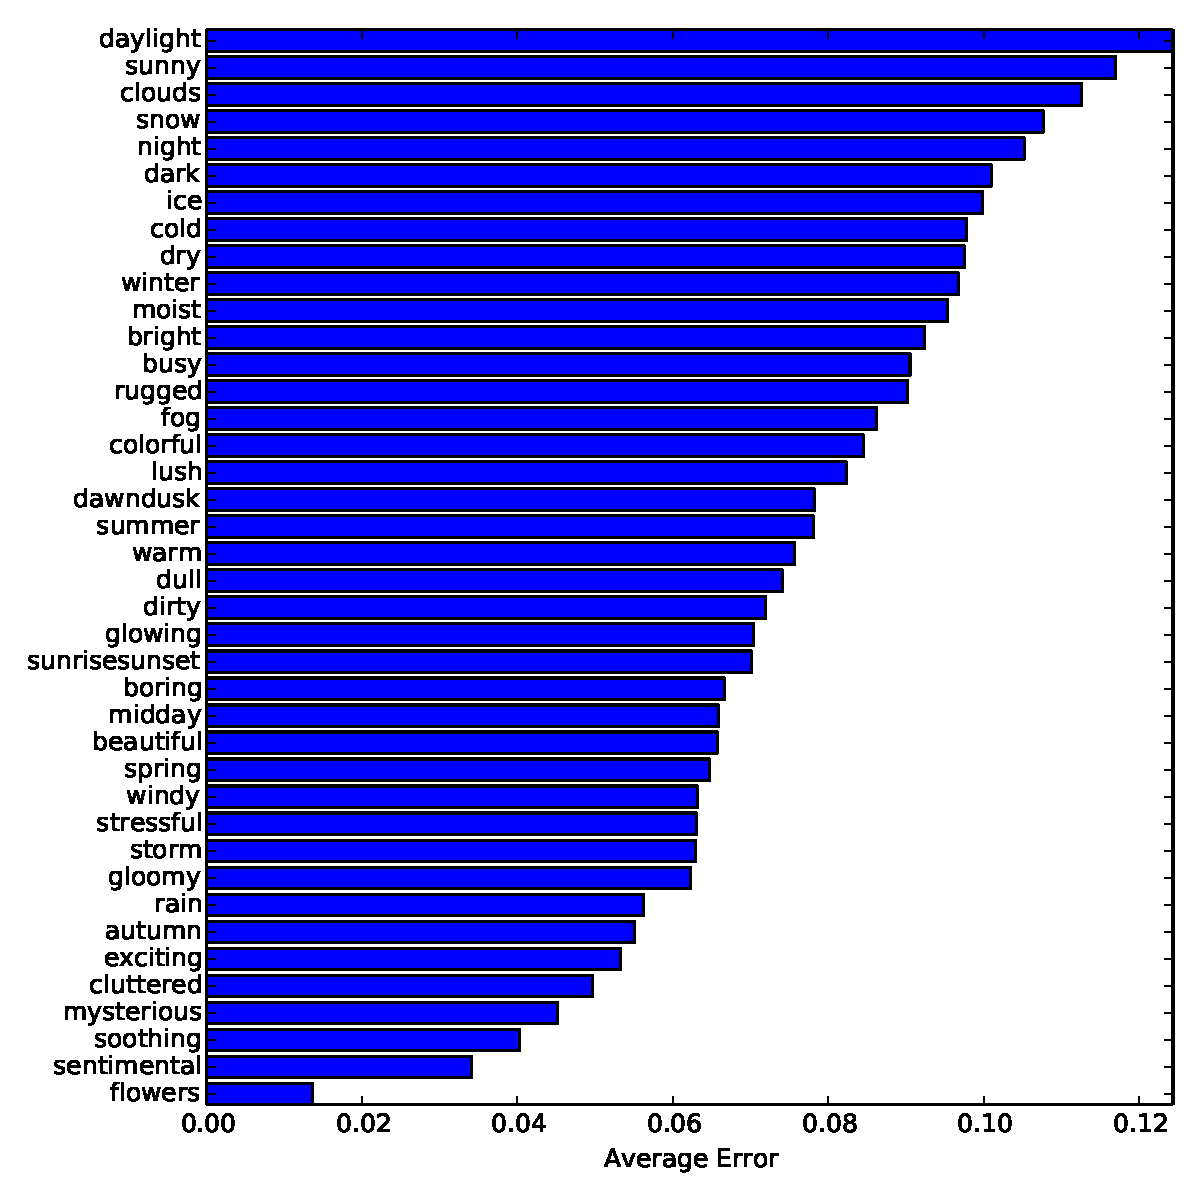
\includegraphics[width=0.5\textwidth]{figs/sorted_err.pdf}
		\caption{Sorted errors from caffenet}\label{fig:sort}
\end{figure}

\begin{figure}[t]
	\centering
		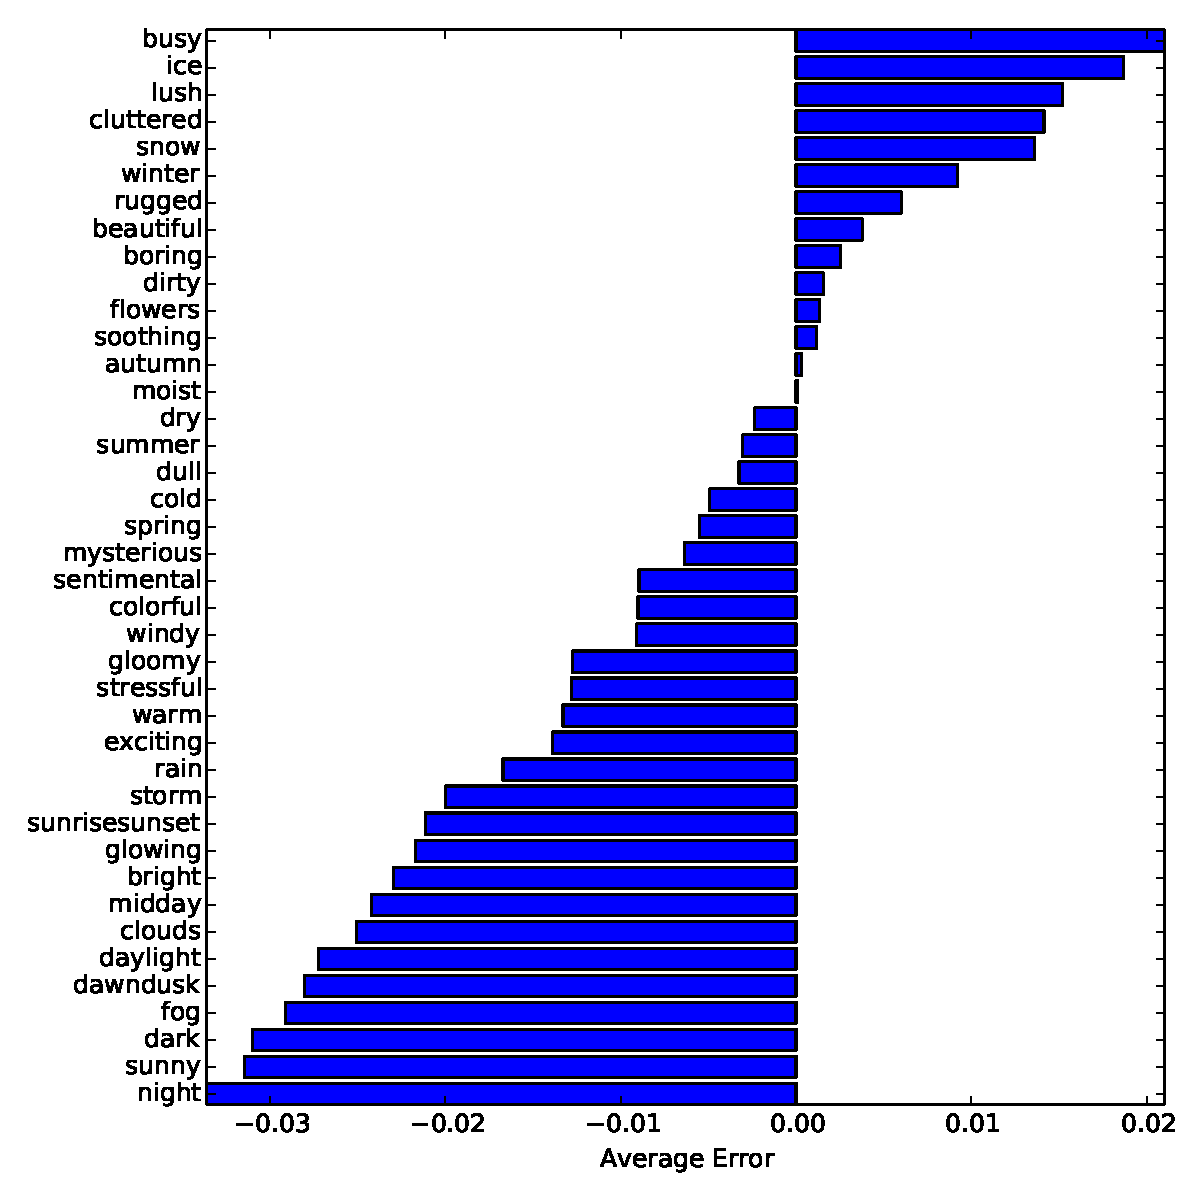
\includegraphics[width=0.5\textwidth]{figs/rel_err.pdf}
		\caption{Relative errors us minus them}\label{fig:relerr}
\end{figure}

\begin{figure*}[t]
	\centering
		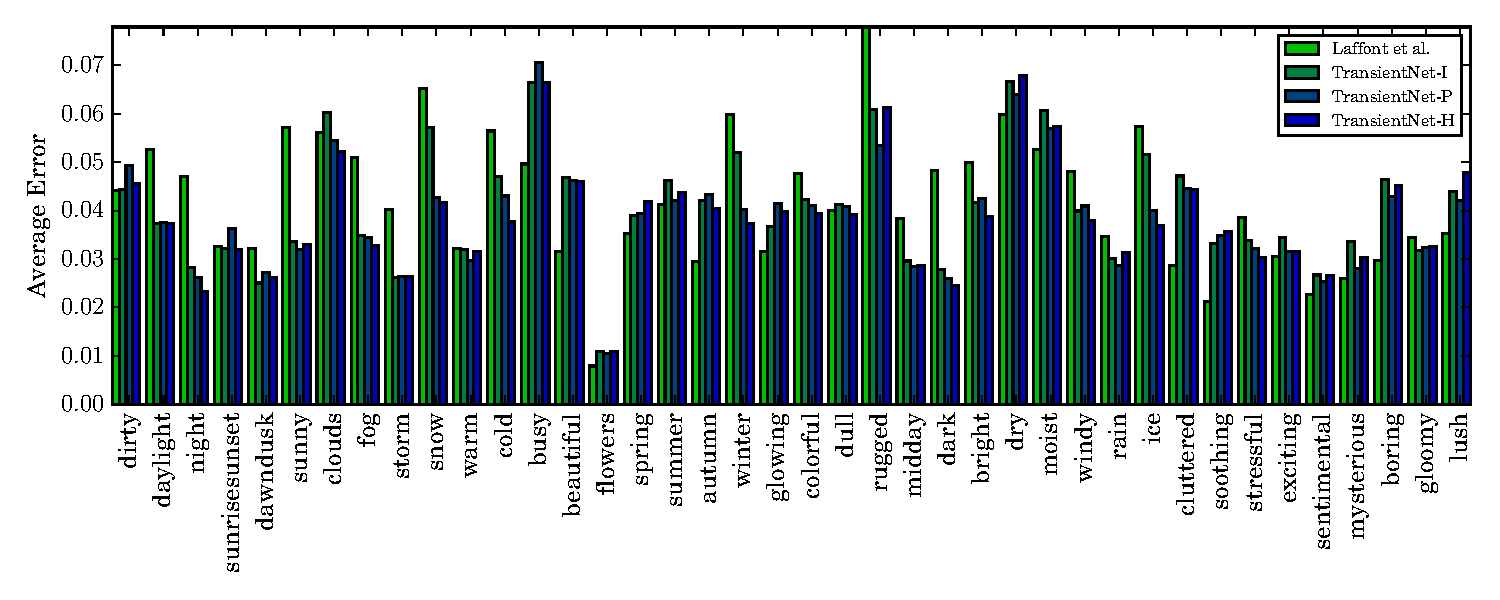
\includegraphics[width=1.0\textwidth]{figs/avg_err_compare.pdf}
		\caption{comparing average errors}\label{fig:compare}
\end{figure*}

\section{Conclusions}

\todo{write me}

more accurate

simpler and easier to train

faster

composable

\bibliographystyle{IEEEbib}
\bibliography{refs}

\end{document}

